\documentclass[a1paper, portrait,innermargin=10mm, blockverticalspace=10mm, colspace=10mm,margin=0mm,]{tikzposter} %,   subcolspace=-5mm
\tikzposterlatexaffectionproofoff



\usepackage{tabulary}
\usepackage{caption}
\usepackage{enumerate}

%\usepackage{cite}
%\usepackage[english]{babel}
%\usepackage[utf8]{inputenc}
\usepackage{amssymb, amsmath}

\usepackage{tkz-graph}

\newtheorem{thm}{Theorem}
%\newtheorem*{lem}{Lemma}
%\newtheorem*{cor}{Corollary}
\newtheorem{rem}{Remark}
%
%\theoremstyle{definition}
\newtheorem{defn}{Definition}
%\newtheorem*{exmp}{Example}
%\newtheorem*{conj}{Conjecture}

\title{Nonrigid labelings of Laman graphs} 
\author{Jan Legersk\'y} 
\institute{ESR 7, Research Institute for Symbolic Computation, JKU Linz, Austria}


\definecolorstyle{Czech} {
\definecolor{colorOne}{HTML}{34888C}%116699		
\definecolor{colorTwo}{HTML}{C1E1DC} 
\definecolor{colorThree}{HTML}{FFF2BE} 
%\definecolor{colorOne}{HTML}{34888C}%116699
%\definecolor{colorTwo}{HTML}{7CAA2D}
%\definecolor{colorThree}{HTML}{F5E356}
%\definecolor{colorOne}{HTML}{4F6457}%116699
%\definecolor{colorTwo}{HTML}{D9B44A}
%\definecolor{colorThree}{HTML}{ACD0C0}
%\definecolor{colorOne}{HTML}{0D5078}%116699
%\definecolor{colorTwo}{HTML}{A2C4D9}
%\definecolor{colorThree}{HTML}{FCF0AD}
}{
     % Background Colors
    \colorlet{backgroundcolor}{colorTwo}
    \colorlet{framecolor}{colorThree}
    % Title Colors
    \colorlet{titlebgcolor}{colorOne}
    \colorlet{titlefgcolor}{white}
    % Block Colors
    \colorlet{blocktitlebgcolor}{white}
    \colorlet{blocktitlefgcolor}{colorOne}
    \colorlet{blockbodybgcolor}{white}
    \colorlet{blockbodyfgcolor}{black}
    % Innerblock Colors
    \colorlet{innerblocktitlebgcolor}{white}
    \colorlet{innerblocktitlefgcolor}{black}
    \colorlet{innerblockbodybgcolor}{colorThree}
    \colorlet{innerblockbodyfgcolor}{black}
    % Note colors
    \colorlet{notefgcolor}{black}
    \colorlet{notebgcolor}{colorThree}
    \colorlet{notefrcolor}{colorThree}
}


\usebackgroundstyle{Default} %Rays
\usetitlestyle{Filled}
\usecolorstyle{Czech}

\useblockstyle[bodyoffsety=12mm]{Slide}
\usenotestyle{Default}



%\settitle{ \centering \vbox{
%%\@titlegraphic\\[\TP@titlegraphictotitledistance] 
%\centering
%\color{titlefgcolor} {\bfseries \Huge \sc \@title \par}
%\vspace*{1em}
%{\huge \@author \par}% \vspace*{1em} {\LARGE \@institute}
%}}

\newcommand{\RR}{\mathbb{R}}
\newcommand{\trcomp}{$\triangle$-component}
\newcommand{\trcomps}{$\triangle$-components}
\newcommand{\cv}[1]{c_v^{(#1)}}


\begin{document}
\maketitle[titletoblockverticalspace=10mm]


\begin{columns} 
\column{0.5}
\block{Abstract}{
\vspace{3mm}
It is well known that Laman graphs characterize minimal planar structures which are rigid for a generic choice of distances between vertices. We focus on a non-generic choice of distances which lead to a nonrigid structure. It appears that there is a connection between these labelings and another edge labeling which is called bidistance. 

We introduce a notion of \trcomps{} which provides tools to determine a bidistance and nonrigid labeling in some cases.
}

\block{Rigidity and Laman graphs}{
%\begin{defn}
%Let $G=(V_G,E_G)$ be a simple graph with a set of vertices $V_G$ and a set of edges $E_G$. 
%\begin{itemize}
%	\item An \emph{embedding} of $G$ is a map $\varepsilon:V_G\rightarrow \RR^2$. 
%	\item  Let $\lambda:E_G\rightarrow \RR_+$ be an edge labeling of $G$. An embedding $\varepsilon$ is \emph{compatible with} $\lambda$ iff $\forall uv=e\in E_G \colon ||\varepsilon(u)-\varepsilon(v)||^2=\lambda(e)$.
%	%\item A labelled graph $(G,\lambda)$ is \emph{realizable} iff it has a compatible embedding.
%	%\item Two embeddings $\varepsilon_1$ and $\varepsilon_2$ are equivalent iff there exists a direct Euclidean isometry $\sigma$ of $\RR^2$ such that $\varepsilon_1=\sigma \circ\varepsilon_2$.
%	\item A labelled graph $(G,\lambda)$ is \emph{rigid} iff the number of embeddings of $G$ compatible with $\lambda$ up to rotations and translations is finite and nonzero. %to equivalence.
%	\item A graph $G$ is \emph{generically rigid} iff $(G,\lambda)$ is rigid for a generic labeling $\lambda$.
%	\item A graph $G$ has a \emph{nonrigid labeling} iff there exists a labeling $\lambda$ such that the number of embeddings of $G$ compatible with $\lambda$ is up to rotations and translations is infinite.
%\end{itemize} 
%\end{defn}

\begin{defn}
Let $G=(V_G,E_G)$ be a simple graph with a~set of vertices $V_G$ and a set of edges $E_G$. 
\begin{itemize}
	\item An \emph{embedding} of $G$ is a map $\varepsilon:V_G\rightarrow \RR^2$. 
	\item  Let $\lambda:E_G\rightarrow \RR_+$ be an edge labeling of $G$. An embedding $\varepsilon$ is \emph{compatible with} $\lambda$ iff  $$\forall uv=e\in E_G \colon ||\varepsilon(u)-\varepsilon(v)||^2=\lambda(e)\,.$$
	%\item A labelled graph $(G,\lambda)$ is \emph{realizable} iff it has a compatible embedding.
	%\item Two embeddings $\varepsilon_1$ and $\varepsilon_2$ are equivalent iff there exists a direct Euclidean isometry $\sigma$ of $\RR^2$ such that $\varepsilon_1=\sigma \circ\varepsilon_2$.
	\item Let $\lambda$ be a labeling of $G$ with at least one compatible embedding. The labeling $\lambda$ is called \emph{rigid} iff the number of embeddings of $G$ compatible with $\lambda$ up to rotations and translations is finite. Otherwise,  $\lambda$ is called \emph{nonrigid}.
%	\item A graph $G$ is \emph{generically rigid} iff $(G,\lambda)$ is rigid for a generic labeling $\lambda$.
%	\item A graph $G$ has a \emph{nonrigid labeling} iff there exists a labeling $\lambda$ such that the number of embeddings of $G$ compatible with $\lambda$ is up to rotations and translations is infinite.
\end{itemize} 
\end{defn}


\begin{tikzfigure}[Rigid and nonrigid labeling of the three-prism graph.]
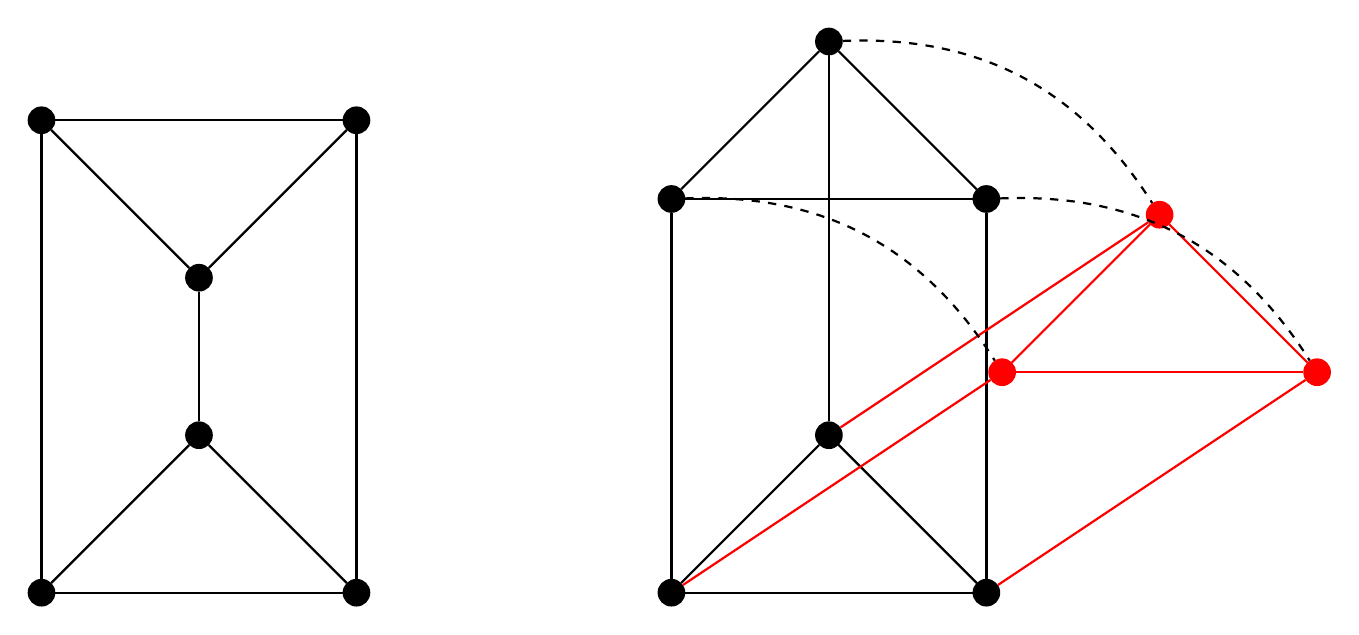
\begin{tikzpicture}
\def \posunx {-8}
\SetVertexNoLabel
   \tikzset{VertexStyle/.style = {shape = circle,fill = black,minimum size = 10pt, inner sep = 0pt}}
   \Vertex[x=0+\posunx ,y=0]{D0}
   \Vertex[x=4+\posunx ,y=0]{E0}
   \Vertex[x=2+\posunx ,y=2]{F0}
   \Vertex[x=0+\posunx ,y=6]{A0}
   \Vertex[x=2+\posunx ,y=4]{C0}
   \Vertex[x=4+\posunx ,y=6]{B0}

%   \tikzset{EdgeStyle/.append style = {}}
   \Edge(D0)(E0)
   \Edge(D0)(F0)
   \Edge(D0)(A0)
   \Edge(F0)(E0)
   \Edge(F0)(C0)
   \Edge(A0)(C0)
   \Edge(A0)(B0)
   \Edge(B0)(E0)
   \Edge(C0)(B0)

%\draw[help lines] (0,0) grid (8,8);
\tikzset{VertexStyle/.style = {shape = circle,fill = black,minimum size = 10pt, inner sep = 0pt}}
   \Vertex[x=0 ,y=0]{D}
   \Vertex[x=4 ,y=0]{E}
   \Vertex[x=2 ,y=2]{F}
   \Vertex[x=0 ,y=5]{A}
   \Vertex[x=2 ,y=7]{C}
   \Vertex[x=4 ,y=5]{B}
   \Edge(D)(E)
   \Edge(D)(F)
   \Edge(D)(A)
   \Edge(F)(E)
   \Edge(F)(C)
   \Edge(A)(C)
   \Edge(A)(B)
   \Edge(B)(E)
   \Edge(C)(B)
\tikzset{VertexStyle/.style = {shape = circle,fill = red,minimum size = 10pt, inner sep = 0pt}}
	\Vertex[x=4.2 , y=3-0.2]{a} 
	\Vertex[x=6.2 , y=5-0.2]{c} 
	\Vertex[x=8.2 , y=3-0.2]{b} 
\tikzset{EdgeStyle/.style = {red}}
	\Edge(a)(D)
   \Edge(F)(c)
   \Edge(a)(c)
   \Edge(a)(b)
   \Edge(b)(E)
   \Edge(c)(b)
\tikzset{EdgeStyle/.style = { dashed, bend left}}
	\Edge(A)(a)
	\Edge(B)(b)
	\Edge(C)(c)
	
\end{tikzpicture}
\end{tikzfigure}
%\begin{thm}
%REFERENCE A graph $G$ is generically rigid iff it is so called \emph{Laman graph} that means
%\begin{itemize}
%	\item $|E_G|=2|V_G|-3$ and
%	\item $|E_H|\leq 2|V_H|-3$ for every subgraph $H$ of $G$. 
%\end{itemize}  
%\end{thm}
\begin{thm}[Laman]
A generic labeling of a graph $G$ is rigid iff $G$ is \emph{Laman graph}, that means
\begin{itemize}
	\item $|E_G|=2|V_G|-3$ and
	\item $|E_H|\leq 2|V_H|-3$ for every subgraph $H$ of $G$. 
\end{itemize}  
\end{thm}
}
\block{Bidistance}{
\begin{defn}
\emph{A bidistance} of a graph $G$ is an edge labeling $\delta:E_G\rightarrow \{0,1\}$ such that for every cycle in $G$, neither 0 or 1 occurs exactly once. A bidistance is \emph{nontrivial} iff $\delta(E_G)=\{0,1\}$.
\end{defn}
\vspace{1.33mm}
\begin{thm}[Schicho]
If a connected graph $G$ has a nonrigid labeling, then it has a nontrivial bidistance.
\end{thm}
%\begin{tikzfigure}[Rigid an nonrigid realization OR EMBEDDING?? of three-prism graph]
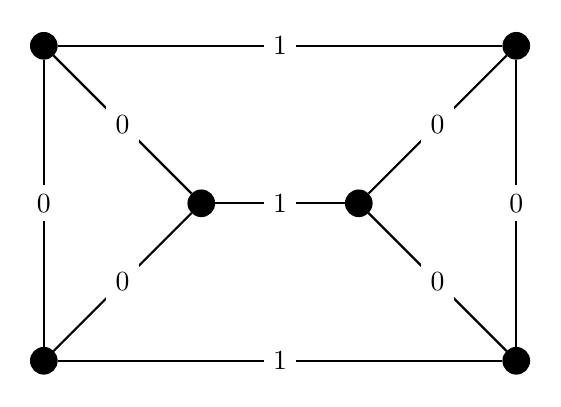
\begin{tikzpicture}
\def \posunx {0}
\SetVertexNoLabel
   \tikzset{VertexStyle/.style = {shape = circle,fill = black,minimum size = 10pt, inner sep = 0pt}}
   \Vertex[x=0+\posunx ,y=0]{D0}
   \Vertex[x=0+\posunx ,y=4]{E0}
   \Vertex[x=2+\posunx ,y=2]{F0}
   \Vertex[x=6+\posunx ,y=0]{A0}
   \Vertex[x=4+\posunx ,y=2]{C0}
   \Vertex[x=6+\posunx ,y=4]{B0}

%   \tikzset{EdgeStyle/.append style = {}}
   \Edge[label=0](D0)(E0)
   \Edge[label=0](D0)(F0)
   \Edge[label=1](D0)(A0)
   \Edge[label=0](F0)(E0)
   \Edge[label=1](F0)(C0)
   \Edge[label=0](A0)(C0)
   \Edge[label=0](A0)(B0)
   \Edge[label=1](B0)(E0)
   \Edge[label=0](C0)(B0)

\end{tikzpicture}
\end{tikzfigure}
}

%\block{DO NOT USE EASY CASE}{
%\begin{thm}
%\label{thm:vertexNotInTriangle}
%Let $G=(V,E)$ be a connected graph such that $|V|\geq 3$. If there is a vertex $v_0 \in V$ such that it is not contained in any triangle $C_3\subset G$, then $G$ allows a nontrivial bidistance. Moreover, $G$ has a nonrigid labeling.
%\end{thm}
%PICTURE OF K3,3?
%}



\column{0.5}
\block{\trcomps{}}{
\begin{defn}
Let $G$ be a connected graph. % such that all vertices are in some triangle $C_3\subset G$. 
We define a relation on $E_G\times E_G$ by 
$$e_1 \sim_{\!\!\bigtriangleup} e_2 \iff  \exists\, C_3\subset G: e_1, e_2\in C_3\,.$$
Let $E_1, \dots, E_n$ be equivalence classes of the reflexive and transitive closure of $\sim_{\!\!\bigtriangleup}$ on $E_G$. The subgraph $T_i=(V_i,E_i)$ of $G$, where  $V_i=\{v\in V | \exists\, e\in E_i \colon v\in e\}$, is called a \emph{\trcomp{} (triangle-component)} iff $|E_i|\geq 3$, and a \emph{connecting edge} otherwise. %A vertex is called \emph{connecting vertex} if it contained in more than one \trcomps{} or connecting edges.
\end{defn}
%\coloredbox{
\begin{tikzfigure}
\begin{tikzpicture}
\def \posunx {0}
\SetVertexLabelOut
   \tikzset{VertexStyle/.style = {shape = circle,fill = niceGreen,minimum size = 10pt, inner sep = 0pt}}
   \SetVertexNoLabel
   \Vertex[x=-.5+\posunx ,y=2.75]{a}
   \Vertex[x=1+\posunx ,y=2]{b}
   \tikzset{VertexStyle/.append style = {fill=red}}   
   \Vertex[x=3+\posunx ,y=2]{c}
   \Vertex[x=4.5+\posunx ,y=2.75]{d}
   \tikzset{VertexStyle/.append style = {fill=blue}}   
   \Vertex[x=0+\posunx ,y=0]{e}
   \Vertex[x=4+\posunx ,y=0]{f}
   \Vertex[x=2+\posunx ,y=4]{v}

   \tikzset{EdgeStyle/.append style = {color=niceGreen}}
	\Edge(a)(e)
	\Edge(e)(b)
	\Edge(a)(b)
	\Edge(b)(v)
	\Edge(a)(v)
	\tikzset{EdgeStyle/.append style = {color=black}}
	\Edge(e)(f)

	\tikzset{EdgeStyle/.append style = {color=red}}
	\Edge(c)(f)
	\Edge(d)(f)
	\Edge(c)(d)
	\Edge(c)(v)
	\Edge(d)(v)
\end{tikzpicture}\hspace{2cm}\parbox[b]{15cm}{\small Fig.~2: A graph with two \trcomps{} ({\color{red} red}, {\color{niceGreen} green}) and one connecting edge (black). The {\color{blue} blue} vertices are so called \emph{connecting vertices}.
}
\end{tikzfigure}
A \trcomp{} has no nontrivial bidistance and hence no nonrigid labeling.
%}
%\begin{defn}
%A vertex $v\in V$ is called \emph{multiple vertex of multiplicity} $k$ if there exists exactly $k$ distinct \trcomps{} which contain $v$. A vertex $u\in V$ is called \emph{connecting vertex} if it is a multiple vertex or an endpoint of some connecting edge.
%\end{defn}
%\begin{thm}
%Let $T$ be a \trcomp{} of a graph $G$. The following statements hold:
%\begin{itemize}
%	%\item $|E_T|\geq 2|V_T|-3$.
%%	\item If $\delta$ is a bidistance of $G$, then for all $e,e'\in E_T$, $\delta(e)=\delta(e')$.
%	\item The \trcomp{} $T$ has no nontrivial bidistance and hence no nonrigid labeling.
%%	\item The \trcomp{} $T$ is a Laman graph iff it is a 2-tree. (A graph $G$ is called \emph{a 2-tree}, if either $G$ is only one edge, or there exist a vertex $v\in V_G$ of degree two, whose neighbours are adjacent and $G\setminus v$ is a 2-tree.)
%\end{itemize}
%\end{thm}
%\begin{rem}
%A \trcomp{} has no nontrivial bidistance and hence no nonrigid labeling.
%\end{rem}
%\begin{thm}
%Let $G$ be a Laman graph with $n$ \trcomp{}.  The following statements hold:
%\begin{itemize}
%	\item Every \trcomp{} is a planar Laman graph.
%	%\item There is no connecting edge with both endpoints in the same \trcomp{}.
%	%\item Any two \trcomps{} can be connected by at most three connecting edges or by one multiple vertex with possibly one connecting edge. If there are three connecting edges, then all three cannot have a common vertex.
%	\item If $c_e$ is the number of all connecting edges in $G$ and $\cv{k}$ is the number of multiple vertices of multiplicity $k$ in $G$, then
%$$
%3(n-1)=c_e + 2\sum_{k=2}^n \cv{k}(k-1)\,.
%$$
%\end{itemize}
%\end{thm}
}



\block{Sufficient conditions}{
\begin{thm}
\label{thm:suffCond}
A Laman graph $G$ with $n$ \trcomps{} has a nonrigid labeling and nontrivial bidistance if some of the following conditions holds:
\begin{itemize}
	\item There is a vertex which is not in any \trcomp{}. 
%	\item ?? The number of all connecting edges is at least $n$.
%	\item There exists a \trcomp{} in $G$ whose connecting vertices are pairwise nonadjacent.
%	\item There are two distinct \trcomps{} which have only two connecting vertices and they are connected by one of them.
%	\item There is a \trcomp{} connected only with one multiple vertex and one connecting edge.
%	\item ?? There are three \trcomps{} which are pairwise connected by a multiple vertex.
	\item There is a set  $E_{c}$ of connecting edges of $G$ such that $G\setminus E_c$ is disconnected.
	\item There is a set  $V_{c}$ of pairwise non-adjacent connecting vertices of $G$ such that $G\setminus V_c$ is disconnected.
%	\item There are two \trcomps{} connected by three connecting edges or by a multiple vertex and connecting edge.
\end{itemize}
\end{thm}	
\vspace{0.7mm}
\begin{tikzfigure}[????????????????//]
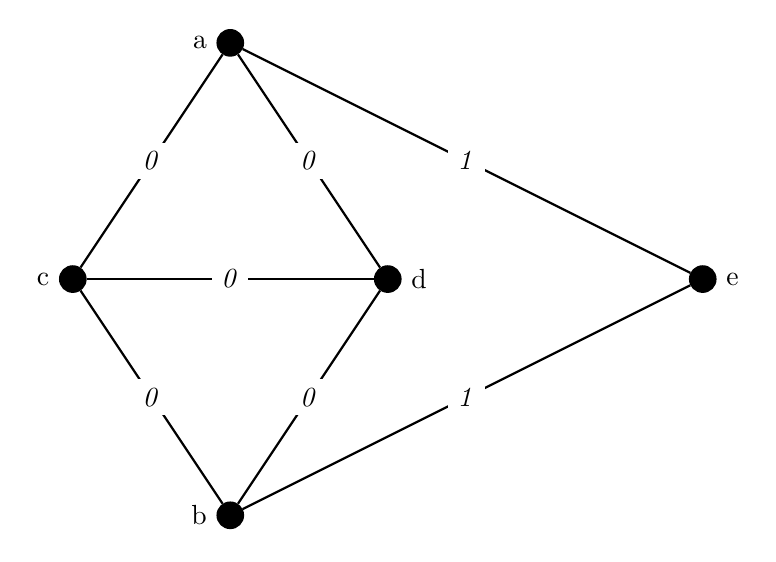
\begin{tikzpicture}
\def \posunx {0}
%\SetVertexNoLabel
\SetVertexLabelOut
   \tikzset{VertexStyle/.style = {shape = circle,fill = black,minimum size = 10pt, inner sep = 0pt}}
   \Vertex[x=0+\posunx ,y=0,Lpos=180]{c}
   \Vertex[x=4+\posunx ,y=0]{d}
   \Vertex[x=2+\posunx ,y=3,Lpos=180]{a}
   \Vertex[x=2+\posunx ,y=-3, Lpos=180]{b}
   \Vertex[x=8+\posunx ,y=0]{e}

%   \tikzset{EdgeStyle/.append style = {}}
	\Edge[label=\emph{0}](a)(c)
	\Edge[label=\emph{0}](c)(b)
	\Edge[label=\emph{0}](a)(d)
	\Edge[label=\emph{0}](c)(d)
	\Edge[label=\emph{0}](b)(d)
	\Edge[label=\emph{1}](a)(e)
	\Edge[label=\emph{1}](b)(e)
%
%%\draw[help lines] (0,0) grid (8,8);
%\tikzset{VertexStyle/.style = {shape = circle,fill = black,minimum size = 10pt, inner sep = 0pt}}
%   \Vertex[x=0 ,y=0]{D}
%   \Vertex[x=4 ,y=0]{E}
%   \Vertex[x=2 ,y=2]{F}
%   \Vertex[x=0 ,y=5]{A}
%   \Vertex[x=2 ,y=7]{C}
%   \Vertex[x=4 ,y=5]{B}
%   \Edge(D)(E)
%   \Edge(D)(F)
%   \Edge(D)(A)
%   \Edge(F)(E)
%   \Edge(F)(C)
%   \Edge(A)(C)
%   \Edge(A)(B)
%   \Edge(B)(E)
%   \Edge(C)(B)
%\tikzset{VertexStyle/.style = {shape = circle,fill = red,minimum size = 10pt, inner sep = 0pt}}
%	\Vertex[x=4.2 , y=3-0.2]{a} 
%	\Vertex[x=6.2 , y=5-0.2]{c} 
%	\Vertex[x=8.2 , y=3-0.2]{b} 
%\tikzset{EdgeStyle/.style = {red}}
%	\Edge(a)(D)
%   \Edge(F)(c)
%   \Edge(a)(c)
%   \Edge(a)(b)
%   \Edge(b)(E)
%   \Edge(c)(b)
%\tikzset{EdgeStyle/.style = { dashed, bend left}}
%	\Edge(A)(a)
%	\Edge(B)(b)
%	\Edge(C)(c)
%	
%\def \posunx {10}
%\SetVertexNoLabel
%   \tikzset{VertexStyle/.style = {shape = circle,fill = black,minimum size = 10pt, inner sep = 0pt}}
%   \Vertex[x=0+\posunx ,y=0]{D0}
%   \Vertex[x=4+\posunx ,y=0]{E0}
%   \Vertex[x=2+\posunx ,y=2]{F0}
%   \Vertex[x=0+\posunx ,y=6]{A0}
%   \Vertex[x=2+\posunx ,y=4]{C0}
%   \Vertex[x=4+\posunx ,y=6]{B0}
%
%   \tikzset{EdgeStyle/.style = {}}
%   \Edge[label=0](D0)(E0)
%   \Edge[label=0](D0)(F0)
%   \Edge[label=1](D0)(A0)
%   \Edge[label=0](F0)(E0)
%   \Edge[label=1](F0)(C0)
%   \Edge[label=0](A0)(C0)
%   \Edge[label=0](A0)(B0)
%   \Edge[label=1](B0)(E0)
%   \Edge[label=0](C0)(B0)
\end{tikzpicture}
\end{tikzfigure}
}

\block{Conjecture}{
\emph{
Let $G$ be a Laman graph with all vertices in a \trcomp{}. The following statements are equivalent:
\begin{enumerate}[i)]
	\item The graph $G$ has a nonrigid labeling.
	\item The graph $G$ allows a nontrivial bidistance.
	\item There are at least two \trcomps{} in $G$.
\end{enumerate}}
Only a proof of $iii) \implies i)$ is missing.
}

\end{columns}

\begin{columns} 
\column{1}
\block{}{\vspace{-5mm}
\begin{minipage}[t]{0.33\colwidth}
	\begin{center}
	\raisebox{0pt}{
	\raisebox{-0.5\height}{
\includegraphics[scale=0.75]{logos/EU.jpg}\hspace{20mm} }
	\raisebox{-0.5\height}{
\includegraphics[scale=0.12]{logos/ARCADES.png} }
	}
	\end{center}
\end{minipage}
\begin{minipage}[t]{0.33\colwidth}\vspace{-10mm}
	\small \center 	This project has received funding from the European Union's Horizon 2020 research and innovation
	programme under the Marie Sk\l{}odowska-Curie grant agreement No 675789.
\end{minipage}
\begin{minipage}[t]{0.33\colwidth}
\begin{center}
	\raisebox{-0.5\height}{
\includegraphics[scale=0.8]{logos/RISC.png}\hspace{20mm}}
\raisebox{-0.5\height}{	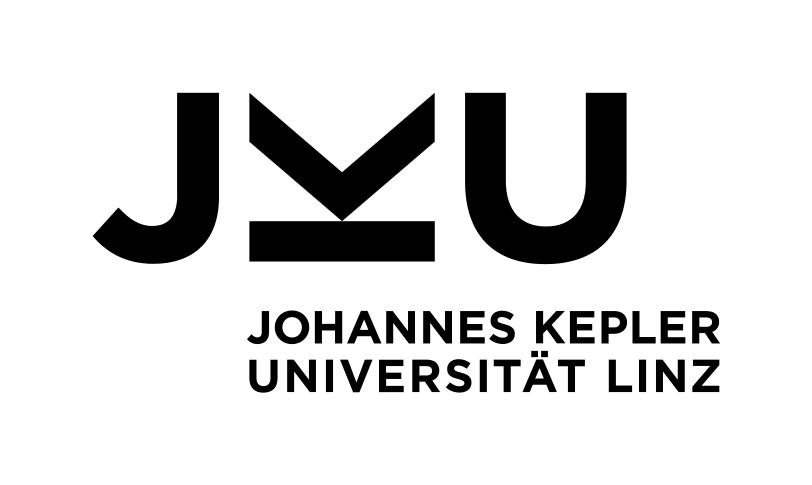
\includegraphics[scale=0.2]{logos/JKU.png}}
	\end{center}
\end{minipage}
}
\end{columns}
\end{document}


